\section{Subsidiando el transporte}

\subsection{Descripción del problema}
En este problema, observamos la provincia de Optilandia, cuyas ciudades estan conectadas por rutas de una sola dirección, donde no necesariamente se puede llegar de una ciudad a todas las demás. Sin embargo, sabemos que desde cualquier ciudad se puede llegar, al menos, a otra ciudad. Cada una de estas rutas tiene una cabina de peaje y, por ende, recorrer cada una de ellas tiene un costo. Sin embargo, por decisiones gubernamentales, cada uno de estos peajes se vio reducido por un costo fijo c (si antes la ruta A valía A1, y la ruta B valía B1, ahora valen A1 - c y B1 - c respectivamente), pudiendo generar que una ruta no solo no le cobre a sus usuarios, sino que acabe dándole dinero.
\\
\par
Si bien esto no es un problema para el gobierno, siempre y cuando se evite que un usuario pueda irse desde una ciudad, hacer un recorrido y volver a la misma habiendo ganado plata. Por lo tanto, como el gobierno busca maximizar el subsidio otorgado, debemos buscar el valor c que permita otorgar el mayor subsidio por peaje sin que exista la posibilidad de que un usuario le saque plata al Estado. La complejidad del algoritmo debe ser no peor que \textbf{O($nm.log(c)$)}, donde n es la cantidad de ciudades, m es la cantidad de rutas y c es el costo del máximo peaje
\\
\par
Veamos un ejemplo del problema. Supongamos que tuvieramos 6 ciudades, con las siguientes rutas iniciales y con los siguientes costos de peaje1 expresados en pesos:
\begin{itemize}
\item Ruta de 1 a 2. Costo de peaje: 40 pesos.
\item Ruta de 2 a 3. Costo de peaje: 20 pesos.
\item Ruta de 3 a 4. Costo de peaje: 10 pesos.
\item Ruta de 4 a 1. Costo de peaje: 15 pesos.
\item Ruta de 5 a 2. Costo de peaje: 5 pesos.
\item Ruta de 6 a 3. Costo de peaje: 10 pesos.
\end{itemize}

Como vemos, la única manera de salir de una ciudad y volver a la misma es que arranquemos en las ciudades 1, 2, 3 ó 4, y recorramos las cuatro rutas que las conectan. Por ende, debemos asegurar que al recorrerlas no se le saca plata al estado; es decir, que al aplicarle el subsidio fijo, se descuenta menos de (40+20+10+15) $=$ 85 pesos. Considerando que las cuatro rutas tienen el mismo descuento, el mayor subsidio que se podría realizar es la cuarta parte de 85, que si lo redondeamos es 21 pesos. Por lo tanto, el mayor descuento que se podría realizar a las rutas de esta provincia es de 21 pesos.
\\
\par
\subsection{Desarrollo}
Dado este problema, y considerando que hay que tener en cuenta la mano en la cual corren las rutas, la mejor manera de modelarlo sería utilizando digrafos. Así, cada ciudad se representaría con un nodo, y cada una de las rutas que conecta dos ciudades, con una arista dirigida. Consideraremos que un recorrido abusivo es representado por un ciclo negativo en el digrafo.
\\
\par
Como nuestro problema principal es averiguar cual es el mayor subsidio que se le puede otorgar a todas las rutas sin que se generen ciclos de rutas negativos, no es dificil que rápidamente encontremos una visión certera de lo que debemos hacer en el problema. Como primer aproximamiento, podemos asegurar que nuestro objetivo será reducir el costo de las rutas de manera que vayamos obteniendo mejores valores hasta que, superado el valor máximo, encontremos ciclos negativos en nuestro grafo.
\\
\par
Por ende, sabemos de entrada que necesitaremos un algoritmo capaz de reconocer ciclos negativos; y considerando los límites de complejidad brindados, podemos asegurarnos que Bellman-Ford cumple nuestros propositos. Esto nos permitirá utilizar aristas negativas, y averiguar en cada uno de los nodos si en sus componentes hay o no ciclos negativas.
\\
\par
Dado que en el problema original queremos detectar la existencia de ciclos negativos para distintas versiones del mismo grafo, usamos una función que permite crear una nueva versión del grafo a partir del original. Diremos que una p-versión nueva del grafo contiene la misma cantidad de nodos y representa al mismo conjunto de adyacencias, y su diferencia radica en que para todo eje de u a v con peso w perteneciente al grafo original, hay un eje de u a v con peso (w-p) perteneciente a la p-versión. Así, utilizaremos un algoritmo que, para cada versión, nos diga si efectivamente al aplicarle Bellman Ford se encuentran o no ciclos negativos (para esto, suponemos que Bellman-Ford nos devuelve $true$ si encuentra ciclos negativos, y $false$ si no lo hace)
\\
\par
\begin{algorithm}[H]
		\NoCaptionOfAlgo
		\caption{\algoritmo{ajusteParaBellmanFord}{\In{p}{int}, \In{ejesGrafo}{lista[ejes]}, \In{origen}{int}}{bool}}
		
		lista[ejes] ejesPVersion $\leftarrow$ ajustarEjes(ejesGrafo, p)\\
		res $\leftarrow$ bellmanFord(ejesPVersion, origen)\\

	\end{algorithm}

Diremos que c es el peso de la arista mas pesada del grafo original. Veamos que la versión p $=$ 0 es equivalente al grafo original, y por ende no puede tener ciclos negativos. Por otro lado, veamos que si el grafo original tiene ciclos, la versión p $=$ c + 1 tendrá ciclos negativos, porque todas sus aristas necesariamente lo tendrán. Por ende, sabemos que nuestra solución esta acotada inferiormente por 0 y superiormente por c.
\\
\par
Por otro lado, teniendo en cuenta un Q cualquiera, sabemos que si la versión Q carece de ciclos negativos entonces toda versión con un valor de subsidio menor a Q también carecerá de ellos. La intuición aquí reside en notar que aumentar el peso de cada arista de un grafo sin ciclos negativos producirá el aumento del peso del ciclo, y por lo tanto, que se mantenga por arriba de 0. Y del mismo modo, podemos notar lo inverso: si la versión Q posee ciclos negativos, toda versión con un valor de subsidio mayor a Q los contendrá.
\\
\par
Entonces, sabiendo que un valor Q bien nos habla de todos los mayores o menores a él; y considerando que nuestra solución se encuentra entre 0 y c, podemos realizar una búsqueda binaria tal que para cada versión Q, si la misma posee ciclos negativos, nuestra solución se acotará entre 0 y Q. En cambio, si no los posee, su solución se encontrará entre Q y c.
\\
\par
Dado que Bellman-Ford solo puede detectar ciclos negativos en digrafos si son fuertemente conexos, y sabiendo que el grafo de entrada no necesariamente cumple tal hipótesis, será necesario realizar un preprocesamiento al grafo de entrada. Para esto, diremos que un nodo v es huérfano si y solo si $d_{in} (v) = 0$.
\\
\par
Dado que ningún nodo puede llegar a un nodo huérfano, y que en un grafo fuertemente conexo debe existir un camino de ida y de vuelta entre todo par de nodos, si un digrafo contiene nodos huérfanos no es fuertemente conexo. Por el mismo motivo, dado que los nodos huérfanos tampoco pueden pertenecer a un ciclo dirigido, no son relevantes en nuestra bísqueda de ciclos. Entonces, podemos contemplar el grafo donde no hay nodos huérfanos, simplemente aislándolos del resto del digrafo, y eliminando todos sus ejes de salida. Sin embargo, al eliminar los ejes de un nodo huérfano, estaríamos reduciendo el grado de entrada de sus hijos, pudiendo producir nuevos nodos huérfanos, que también deberían ser aislados.
\\
\par
En síntesis, lo que deberíamos hacer es tomar el grafo actual, y quitar todos los nodos huérfanos del mismo, reiteradas veces hasta que finalmente no haya ningún nodo con $d_{in} (v) = 0$. Por lo tanto, para generar un grafo acorde a nuestros propositos, utilizaremos un algoritmo similar a este:\\
\begin{algorithm}[H]
		\NoCaptionOfAlgo
		\caption{\algoritmo{borrarNodosHuerfanos}{\In{n}{nat}, \In{lista[ejes]}{ejesGrafo}}{}}
		
		lista[nat]: adyacentes $\leftarrow$ listaDeAdyacencia(ejesGrafo)\\
		lista[nat]: gradoEntrada $\leftarrow$ gradoDeEntrada(ejesGrafo)\\
		pila[nat]: nodosHuerfanos $\leftarrow$ vacia()\\
		\While{j $<$ n}{
			\eIf{nodosHuerfanos.esVacia()}{
				\eIf{gradoEntrada[j] $=$ 0}{
					agregarNodosHuerfanos(nodosHuerfanos, adyacentes, gradoEntrada, j, ejesGrafo)\\
					gradoEntrada[j] $\leftarrow$ NULL
					}{j $\leftarrow$ j + 1\\}
				}{
					nat: k $\leftarrow$ nodosHuerfanos.dameTope()\\
					agregarNodosHuerfanos(nodosHuerfanos, adyacentes, gradoEntrada, k, ejesGrafo)\\
					}
		}

	\end{algorithm}


Cuando logramos aislar a todos los nodos huerfanos del digrafo principal, ya estamos en condiciones de asegurar que para todo nodo v, $d_{in} (v) > 0 \land d_{out} (v) > 0$. Sin embargo, a causa de la siguiente propiedad, no es hipótesis suficiente para que el digrafo sea fuertemente conexo:
\\
\par
\begin{center}
Orientar un grafo es darle una dirección a cada eje. Un grafo conexo G es orientable de forma tal que se convierta en un digrafo fuertemente conexo si y sólo si cada eje de G pertenece a un circuito simple de G.
\end{center}

Veamos que los ejes que no pertenecen a un ciclo en el grafo subyacente no pueden pertenecer a un ciclo en el digrafo. Entonces, si el digrafo tiene tales ejes, no es fuertemente conexo. Como esos ejes no pueden pertenecer a un ciclo dirigido, no son importantes en nuestro análisis, y por lo tanto eliminarlos no nos quita soluciones. Por lo tanto, deberemos buscar la manera de quitar estos ejes, para así obtener, finalmente un grafo compuesto por componentes fuertemente conexas.
\\
\par
Para esto, tomaremos nuestro grafo actual (al cual ya le hemos eliminado los nodos huérfanos correspondientes) y consideraremos un bosque generador particular (como bien sabemos, es posible que haya ciclos en el grafo, por lo que es importante marcar que no cambiará el resultado cual es el bosque generador que tomemos). A partir de aquí, tenemos dos tipos de ejes: los que pertenecen al bosque generador, a los cuales llamaremos \textbf{inciertos}, y los cuales no pertenecen.
\\
\par
Como tenemos un bosque generador, si agregamos cualquier arista que conecte dos ejes formaremos un ciclo. Por lo tanto, podemos asegurar que todos los ejes que no pertenezcan al bosque generador son partes de un ciclo de nuestro grafo, y por ende conforman una solución parcial. Sin embargo, aún debemos determinar cuales de las aristas inciertas son las que forman ciclos. Para esto, empezaremos por considerar el grafo que conecta a todas las aristas que ya sabemos útiles (las seleccionadas) y considerar a cada una de ellas como parte de una componente conexa. Es decir que si una arista seleccionada incide al nodo 2 y 3, y otra al nodo 3 y 4, necesariamente serán parte de la misma componente conexa.
\\
\par
Luego, viendo cada una de las aristas inciertas, deberemos recorrer estas componentes; y al encontrar una arista que incide sobre dos nodos de la misma componente, aseguraremos que esta arista es parte de un ciclo (puesto que ya había un camino entre estos dos nodos, por ser parte de la misma componente, y ahora hay un camino nuevo), y por ende, de las aristas que influyen sobre nuestro problema.
\\
\par
Es importante resaltar que, luego de agregar una arista a las seleccionadas, deberemos repasar las aristas inciertas ya recorridas, pues contaremos con un nuevo conjunto de componentes conexas y, por lo tanto, de ciclos. En términos de pseudocódigo, tendríamos algo así:

\begin{algorithm}[H]
		\NoCaptionOfAlgo
		\caption{\algoritmo{subsidioDeRutas}{\Inout{inputEdges}{lista[ejes]}}{}}
		
		bool: changesMade $\leftarrow$ true
		
		lista[ejes]: edgesToUse $\leftarrow$ kruskalParaBosque(inputEdges)

		lista[ejes]: inputEdges $\leftarrow$ inputEdges - edgesToUse

		\While{changesMade} 
		{
			changesMade $\leftarrow$ false

			set: ds $\leftarrow$ $\emptyset$

			\For{(u,v) $\in$ inputEdges}
			{
				ds.join(u, v)
			}

			\For{(u,v) $\in$ edgesToUse}
			{
				\eIf{ds.connected(u,v)}
					{
						inputEdges.add((u,v))

						edgesToUse.erase((u,v))

						changesMade $\leftarrow$ true
					}
					{
						ds.join(u, v)
					}
			}



		}
	\end{algorithm}

Por lo tanto, luego de borrar los nodos huérfanos y asegurarnos que todas las aristas de la última versión del grafo pertenecen a un ciclo, contamos con las siguientes hipotesis: para todo nodo v del grafo, $d_{in} (v) > 0 \land d_{out} (v) > 0 \land$ en el grafo subyacente, v pertenece a al menos un ciclo. Esto alcanza para decir que toda componente conexa es fuertemente conexa. Tomemos dos nodos u, v del grafo. Como ambos pertenecen a la misma componente conexa existe un camino entre ellos. Por hipotesis todos los ejes del camino pertenecen a un ciclo. Si estos ejes estuvieran orientados de manera que no se puede llegar de u a v o de v a u, significaría que hay al menos un nodo w en el camino por el que no se puede pasar, en otras palarbas o bien $d_in(w)$ = 0 o bien $d_out(w)$ = 0. Esto contradice a las hipótesis, absurdo.

Por lo tanto, con lo ya expuesto, podemos utilizar el algoritmo con ajuste de Bellman-Ford que expusimos anteriormente. Sin embargo, como solo podemos asegurarnos que cada una de las componentes conexas de nuestro grafo es fuertemente conexa, deberemos correr este algoritmo para un representante de cada componente. Por otra parte, como sabemos que cada componente, efectivamente, es fuertemente conexa, bastará con que un representante de la componente nos asegure si hay o no ciclos negativos. Por lo tanto, nuestro algoritmo sería algo así:

\begin{algorithm}[H]
		\NoCaptionOfAlgo
		\caption{\algoritmo{subsidioDeRutas}{\In{n}{nat}, \In{ejesGrafo}{lista[ejes]}}{nat}}
		
		borrarNodosHuerfanos(n, ejesGrafo)\\	borrarEjesQueNoFormanCiclo(ejesGrafo)\\
 		nat: cotaInferior $\leftarrow$ 0\\
 		nat: cotaSuperior $\leftarrow$ pesoMax(ejesGrafo)\\
 		\While{cotaInferior $<$ cotaSuperior}{
 		nat: nuevaCota $\leftarrow$ (cotaInferior + cotaSuperior) / 2 \\
 		bool: tieneCiclos $\leftarrow$ ajusteBellmanFord(ejesGrafo, nuevaCota)\\
 		\eIf{tieneCiclos}{
 			cotaSuperior $\leftarrow$ nuevaCota
 			}{
 			cotaInferior $\leftarrow$ nuevaCota
  			}
 	res $\leftarrow$ cotaInferior
 	}
  	\end{algorithm}


\subsection{Cota temporal}
\begin{center}
\textbf{borrarNodosHuerfanos}
\end{center}
\par
Este algoritmo genera, inicialmente, una lista de adyacencia para cada nodo, un vector de n lugares donde el i-ésimo espacio nos dice el grado de entrada del i-ésimo nodo y una pila vacía. Como nos dan la lista de ejes, al recorrerla podemos generar la lista de adyacencia de cada uno de los ejes y, a su vez, ir contando para cada nodo cuantos nodos tienen ejes apuntando hacia él; y puesto que la entrada a ambos vectores es $O(1)$, y agregar un elemento a una lista también, el costo relevante es el de recorres todas las aristas: $O(m)$, donde m son las aristas del grafo.
\\
\par
Por otra parte, tenemos el ciclo que se encarga de recorrer los $n$ nodos y averiguar si efectivamente es un nodo huerfano o no. Como vemos en el algoritmo expuesto arriba, hay un ciclo que se recorre $n$ veces, lo cual nos da una complejidad de $O(n)$. Sin embargo, no es cierto que el valor $j$ aumenta cada vez que corre el ciclo, sino que depende tambien del hecho de que la pila de nodos huerfanos esté vacía.
\\
\par
Como vimos en el desarrollo, esta pila se encarga de recorrer la lista de adyacencia del nodo huerfano que estamos evaluando, con un costo de $O(n)$, donde n son todos los nodos del grafo (el mayor tamaño posible de la lista de adyacencia). Este proceso se puede producir, como mucho, para los $n$ nodos, en caso de que a través de este algoritmo fueramos descubriendo que cada uno de ellos es huérfano. Por lo tanto, la complejidad de esta porción del algoritmo sería $O(n^2)$.
\\
\par
Pero entonces, al repasar el ciclo, nos encontramos que en el peor caso puede llegar a recorrer dos veces la lista. Suponiendo que, efectivamente, terminaramos apilando los $n$ nodos, tendríamos una complejidad de $O(n^2)$; pero por otro lado, de manera ajena a lo que ocurriera en la pila, el valor de $j$ iría aumentando y, en el peor caso, corriendo n veces la función agregarNodosHuerfanos, dándonos una complejidad de $O(n^2)$. Por ende, aún considerando los dos peores casos en simultáneo (es decir, que los $n$ nodos fueran encontrados recorriendo el vector, y a su vez, agregados a la pila) tendríamos $O(n^2 + n^2)$ $\subseteq$ $O(n^2)$

\begin{center}
\textbf{borrarEjesQueNoFormanCiclo}
\end{center}
Este algoritmo utiliza, para empezar, una versión de Kruskal adaptada para bosques, que mantiene el costo original de Kruskal y, por lo tanto, nos cuesta $O(m.log(n))$, donde m es la cantidad de ejes y n la cantidad de aristas, y lo cual resultará despreciable para la complejidad que tiene el algoritmo.
\\
\par
Luego, realiza la iteración de los ejes. Como cada iteración en la que se añaden ejes a los seleccionados conecta al menos a dos componentes de nuestra lista de incidencia, y hay a lo sumo $n$ componentes distintas, el ciclo itera a lo sumo $n$ veces a todos los ejes, realizando para cada eje operaciones de find y unión, lo que nos da una complejidad de $O(n.m)$. Por otra parte, gracias a las optimizaciones de la estructura disjoint set, podemos despreciar el valor de sus operaciones, considerandolas $O(1)$.
\\
\par
Finalmente, nuestro algoritmo definitivo itera de manera binaria, lo cual nos da un ciclo que se recorre $O(log(c))$ veces para la complejidad $O(n.m)$, dándonos, en definitiva, una cota temporal de $O(n.m.log(c))$

\subsection{Experimentacion}

La experimentación de este ejercicio representó un desafío, ya que en la generación de grafos resultó difícil garantizar condiciones que diesen resultados homogéneos debido a nuestra implementación. Esto requeriría crear grafos fuertemente conexos, de modo que ningún eje estuviese fuera de un ciclo. Sin embargo, sí pudimos observar fácilmente los casos de grafos completos.

\begin{center}
	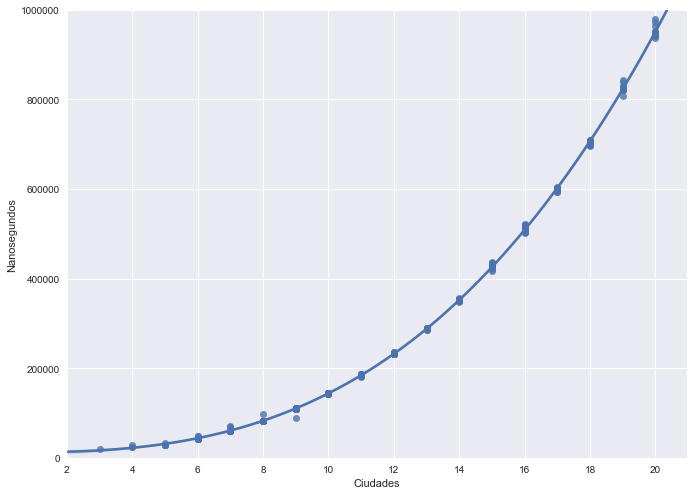
\includegraphics[scale=0.5]{imagenes/ej2-1.png}
\end{center}

En este gráfico se puede observar que, en grafos completos, el algorítmo tiene complejidad cúbica con respecto a la cantidad de ciudades. Esto se ajusta a la complejidad pedida, ya que $m = \frac{n \times (n-1)}{2} \approx n^2$, es decir, $O(n m) \subseteq O(n^3)$.

\begin{center}
	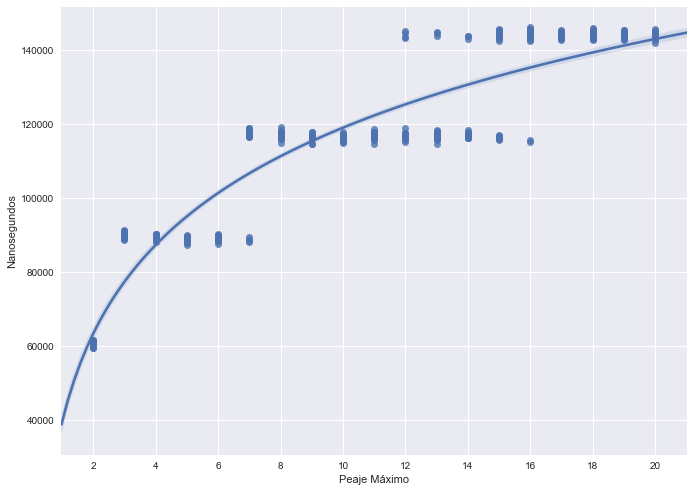
\includegraphics[scale=0.5]{imagenes/ej2-2.png}
\end{center}

Por otro lado, podemos ver que el máximo peaje tiene impacto logarítmico sobre el tiempo de ejecución, lo que condice con nuestras expectativas y con la cota de complejidad pedida. 

\pagebreak